\documentclass[10pt]{article}

\usepackage{commands}
\pgfplotsset{compat=1.18}
\hypersetup{colorlinks = true}

\begin{document}



\section{PHY509 – Problem Set 1}

\subsection*{Problem 1}
\begin{quote}
	Prove that the conditional probability $P(\cdot\mid F)$, for any event $F$ in $S$, is indeed a probability (i.e., satisfies the axioms), where the dot represents the location of the function input. For example, one axiom is $P(S\mid F)=1$.
\end{quote}

\divider

The axioms of probabilities are (partly from lecture 1 and also from \cite{statproofbook2023}):
\begin{enumerate}
	\item Non-negativity: For any event $E\subseteq S$, $P(E)\ge 0$.
	\item Normalization: $P(S)=1$.
	\item Countable additivity: For any countable sequence of disjoint events $E_1,E_2,\ldots$ in $S$,
	      \[
		      P\left(\bigcup_{i=1}^\infty E_i\right) = \sum_{i=1}^\infty P(E_i).
	      \]

	      Take numerator term of conditional probability definition $P(E \cap F)$ and write it in terms of the axiom of countable additivity:

	      \[
		      P\left(\bigcup_{i=1}^\infty (E_i \cap F)\right) = \sum_{i=1}^\infty P(E_i \cap F).
	      \]
\end{enumerate}


The conditional probability is defined as

\begin{equation}
	P(E \mid F) = \frac{P(E \cap F)}{P(F)}
\end{equation}

so we need to show that $P(E \mid F)$ for all $E$ in $S$ satisfies the three axioms above.

\begin{enumerate}
	\item Non-negativity: $P(E \mid F) \ge 0$.

	      We know that F is an event in $S$, so $P(F) >0$ by the original non-negativity axiom of probability. Also, $E \cap F$ (any event E and F occuring) is an event in $S$ (the intersection of two events is also an event), so by the original non-negativity axiom of probability, we have $P(E \cap F) \ge 0$. So together we have a positive denominator and a non-negative numerator, which means that $P(E \mid F) = \dfrac{P(E \cap F)}{P(F)} \ge 0$.

	\item Normalization: $P(S \mid F) = 1$.

	      Given that S is the sample space, we know that $S \cap F = F$ (the intersection of the sample space and any event F is just F). We also know that $P(F) > 0$ since F is an event in S.

	      \[
		      P(S \mid F) = \frac{P(S \cap F)}{P(F)} = \frac{P(F)}{P(F)} = 1.
	      \]

	\item Countable additivity: For any countable sequence of disjoint events $E_1,E_2,\ldots$ in $S$,

	      \[
		      P\left(\bigcup_{i=1}^\infty E_i \mid F\right) = \sum_{i=1}^\infty P(E_i \mid F).
	      \]

	      If the events $E_1,E_2,\ldots$ are disjoint, then the events $E_1 \cap F, E_2 \cap F, \ldots$ are also disjoint (because each of those events are a smaller subset of the original disjoint events -- the requirement for those events is that the E event AND F event occur, so it is a stricter condition). This means that this intersection event is also a countable sequence of disjoint events in $S$ that must follow the axiom.
	      \[
		      P\left(\bigcup_{i=1}^\infty (E_i \cap F)\right) = \sum_{i=1}^\infty P(E_i \cap F).
	      \]

	      Then to retrieve the definition of the conditional probability form, we divide both sides by $P(F)$ (which is positive since F is an event in S):
	      \[
		      \frac{P\left(\bigcup_{i=1}^\infty (E_i \cap F)\right)}{P(F)} = \frac{\sum_{i=1}^\infty P(E_i \cap F)}{P(F)}.
	      \]

	      Showing that the axiom of countable additivity holds for the conditional probability:
	      \[
		      P\left(\bigcup_{i=1}^\infty E_i \mid F\right) = \sum_{i=1}^\infty P(E_i \mid F).
	      \]
\end{enumerate}




\subsection*{Problem 2}
\begin{quote}
	For any three events $E,F,G$, express $P(E\cup F\cup G)$ in terms of the probabilities for $E,F,G$, the pairwise intersections $E\cap F$, $F\cap G$, $E\cap G$, and the triple intersection $E\cap F\cap G$.
\end{quote}

\divider

One of the consequences from the axioms was,

\begin{equation}
	P(A \cup B) = P(A) + P(B) - P(A \cap B)
\end{equation}

This is called the inclusion-exclusion principle. Comes from the fact that when you add $P(A)$ and $P(B)$, you are double counting the intersection $P(A \cap B)$, so you need to subtract it out once.

We can use the same logic in the case of three events. You count the individual events, but then you are double counting the pairwise intersections, so you need to substract one of each of those out. You also triple counted the triple intersection, but since you subtracted out 3 pairwise intersections, you end up with none of the triple intersection, so we need to add it back in once. All this together get's us:

\begin{equation}
	P(E \cup F \cup G) = P(E) + P(F) + P(G) - P(E \cap F) - P(F \cap G) - P(E \cap G) + P(E \cap F \cap G)
\end{equation}

See diagram in figure \ref{fig:venn} from \cite{wiki:inclusion-exclusion}.

\begin{figure}
	\centering
	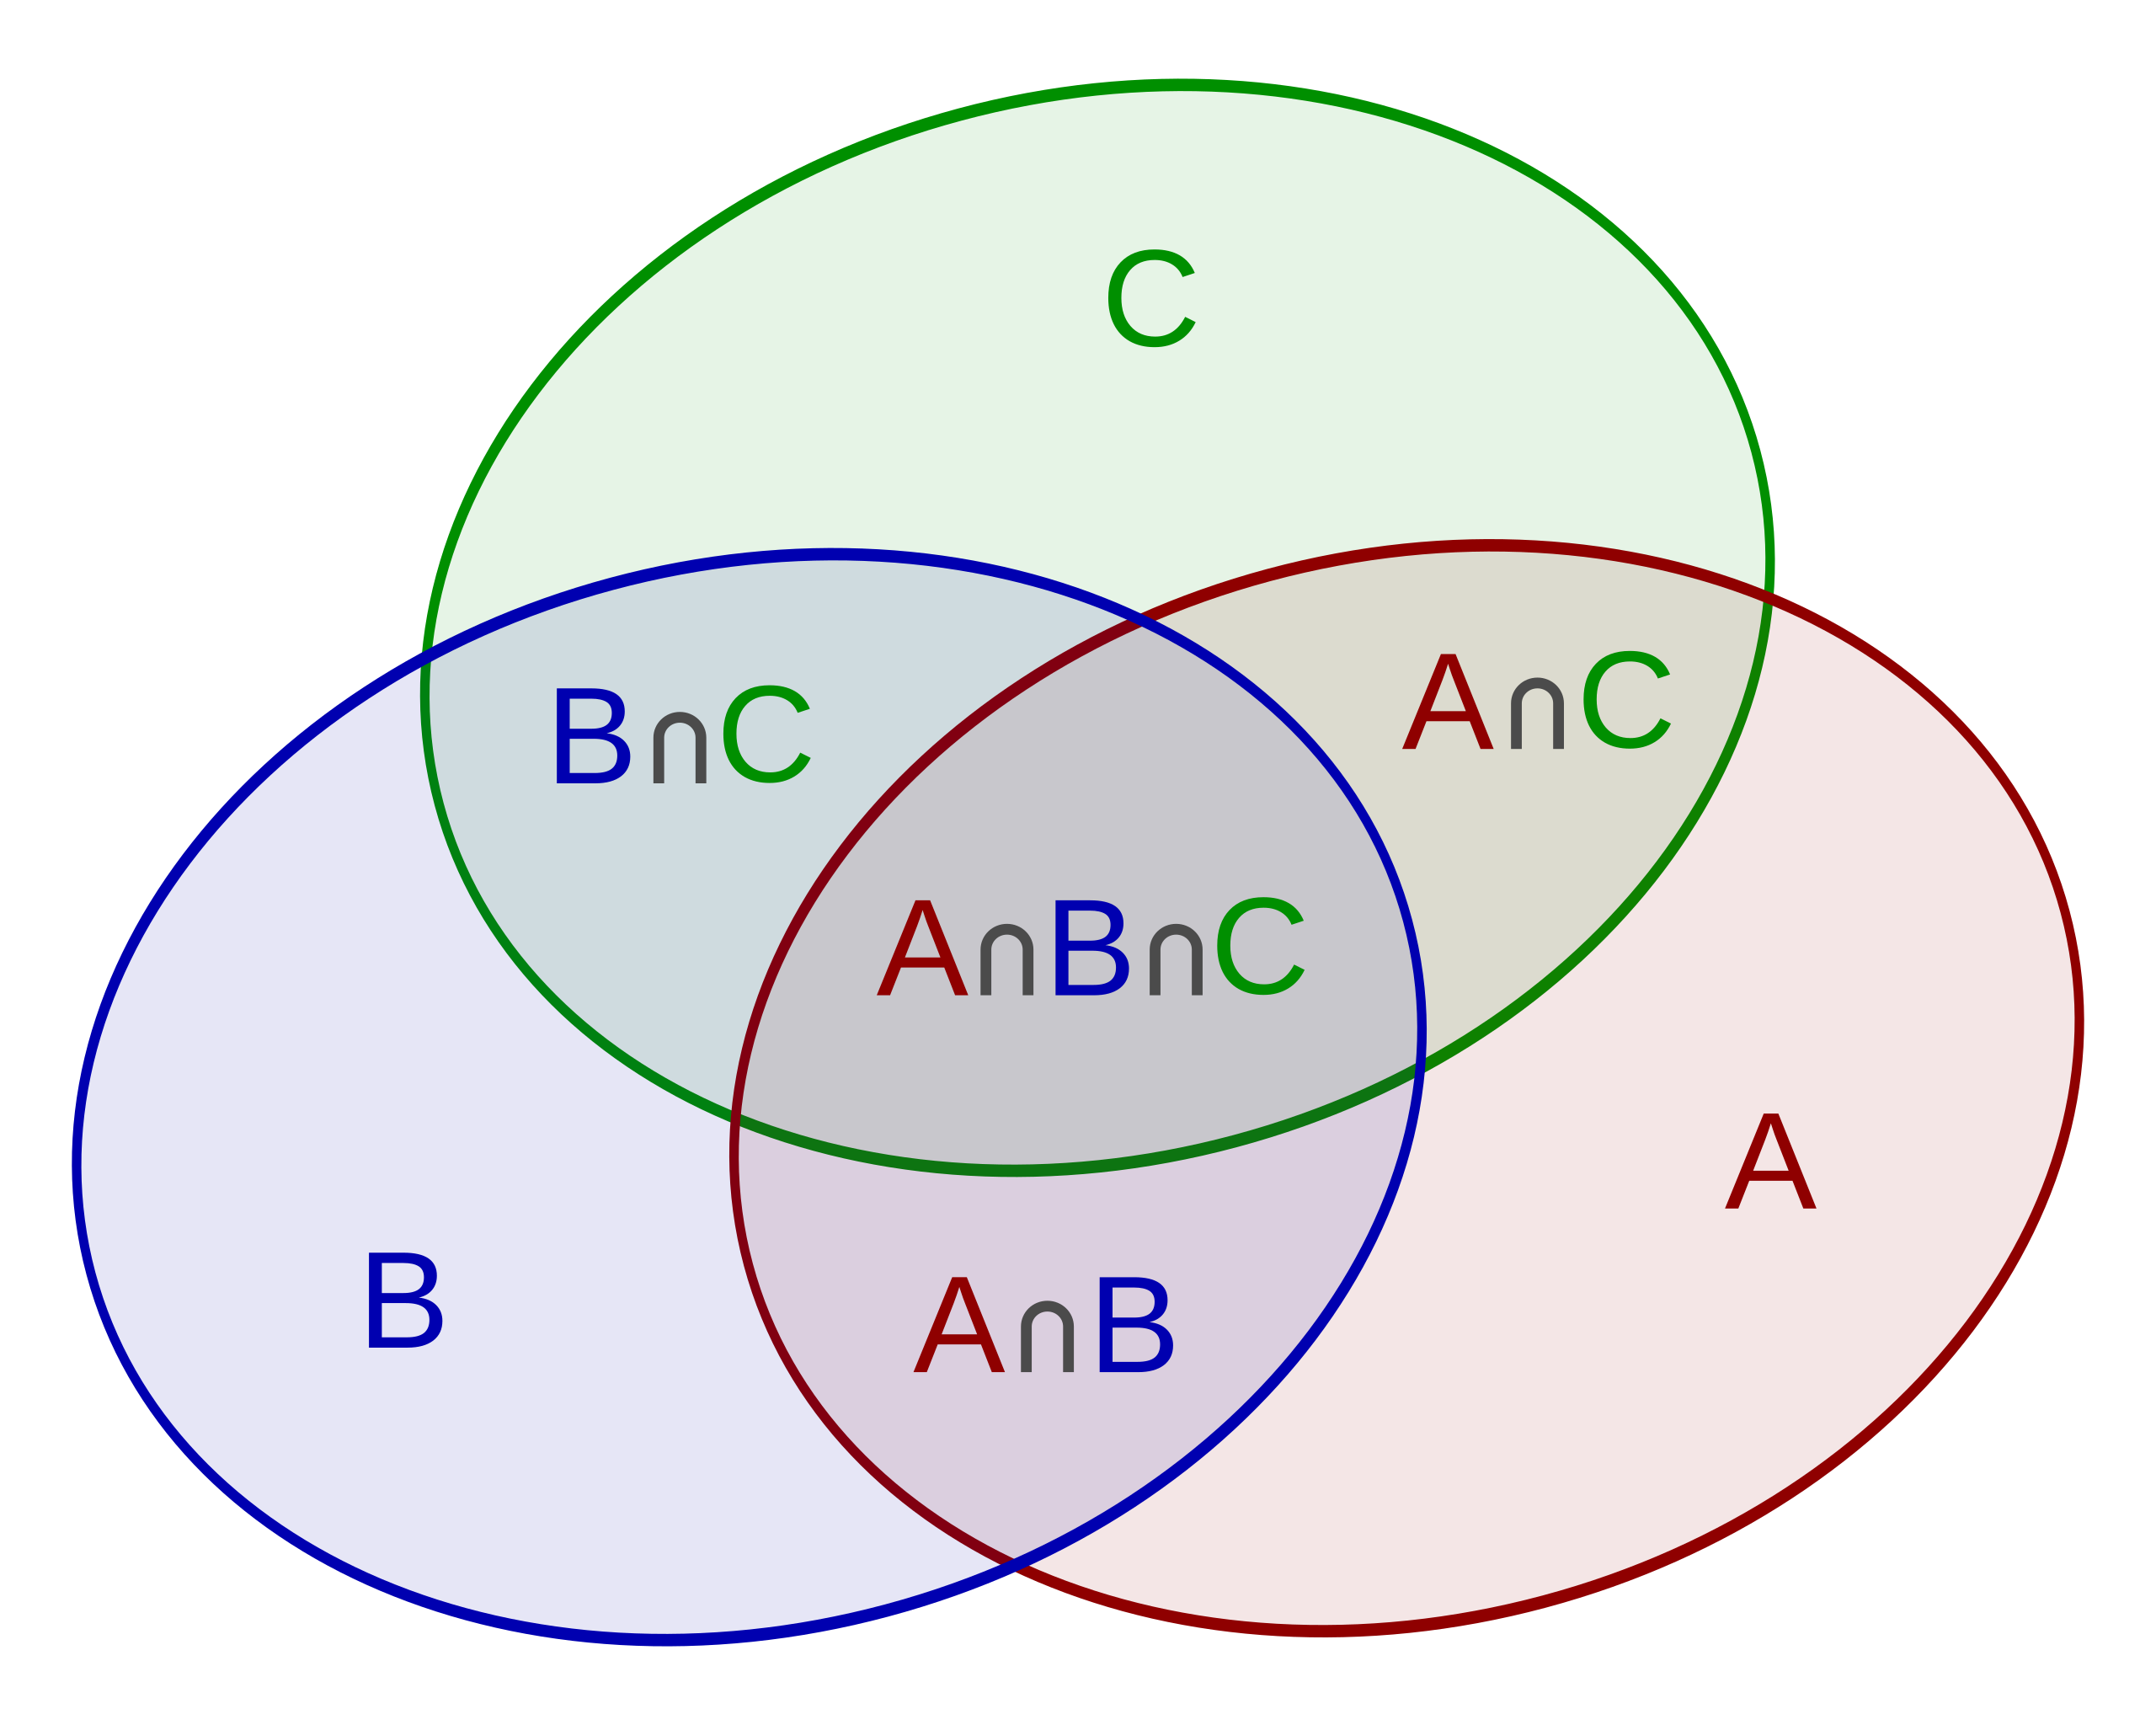
\includegraphics[width=0.5\textwidth]{Inclusion-exclusion.png}
	\caption{Venn diagram for three events.}
	\label{fig:venn}
\end{figure}




\subsection*{Problem 3}
\begin{quote}
	The following data were reported in a study of a group of 1000 people: there were 312 professionals, 470 married persons, 525 college graduates, 42 professional college graduates, 147 married college graduates, 86 married professionals, and 25 married professional college graduates. Show that the numbers reported in the study must be incorrect. Hint: Use the results of the previous problem.
\end{quote}

\divider

If we let $E$ = professionals, $F$ = married persons, and $G$ = college graduates, then we get table \ref{tab:data} from the problem statement.

\begin{table}
	\centering
	\begin{tabular}{|c|c|}
		\hline
		Event                                   & Number of people \\
		\hline
		$E$ = professionals                     & 312              \\
		$F$ = married persons                   & 470              \\
		$G$ = college graduates                 & 525              \\
		$E \cap F$ = married professionals      & 86               \\
		$F \cap G$ = married college graduates  & 147              \\
		$E \cap G$ = professional college grads & 42               \\
		$E \cap F \cap G$ = married prof. grads & 25               \\
		\hline
	\end{tabular}
	\caption{Data from the study.}
	\label{tab:data}
\end{table}

Using the inclusion-exclusion principle from problem 2, we have:

\begin{equation}
	P(E \cup F \cup G) = P(E) + P(F) + P(G) - P(E \cap F) - P(F \cap G) - P(E \cap G) + P(E \cap F \cap G)
\end{equation}

Substituting in the numbers from the table, we get:

\begin{equation}
	P(E \cup F \cup G) = \frac{312}{1000} + \frac{470}{1000} + \frac{525}{1000} - \frac{86}{1000} - \frac{147}{1000} - \frac{42}{1000} + \frac{25}{1000} = \frac{1057}{1000} = 1.057
\end{equation}

This is impossible since the probability of any event must be between 0 and 1, so the numbers reported in the study must be incorrect.

\subsection*{Problem 4}
\begin{quote}
	Let $E,F,G$ be events. Find set expressions for the following events:
	\begin{enumerate}[label=(\alph*)]
		\item only $E$ occurs;
		\item both $E$ and $G$, but not $F$, occur;
		\item at least one of the events occurs;
		\item at least two of the events occur;
		\item all three events occur;
		\item none of the events occur;
		\item at most one of the events occurs;
		\item at most two of the events occur.
	\end{enumerate}
\end{quote}

\divider

Recall our basic set expression notation and rules:
\begin{itemize}
	\item $\cap$ = intersection = AND
	\item $\cup$ = union = OR
	\item $^c$ = complement = NOT
	\item De Morgan's laws:
	      \begin{itemize}
		      \item $(A \cup B)^c = A^c \cap B^c$ : NOT (A OR B) = NOT A AND NOT B
		      \item $(A \cap B)^c = A^c \cup B^c$ : NOT (A AND B) = NOT A OR NOT B
	      \end{itemize}
\end{itemize}

\begin{enumerate}[label=(\alph*)]
	\item $\boxed{E}$ : just E
	\item $\boxed{E \cap G \cap F^c}$ : E AND G AND NOT F
	\item $\boxed{E \cup F \cup G}$ : E OR F OR G
	\item $\boxed{(E \cap F) \cup (F \cap G) \cup (E \cap G)}$ : (E AND F) OR (F AND G) OR (E AND G)
	\item $\boxed{E \cap F \cap G}$ : E AND F AND G
	\item $\boxed{E^c \cap F^c \cap G^c = (E \cup F \cup G)^c}$: NOT E AND NOT F AND NOT G = NOT (E OR F OR G) By De Morgan's law
	\item $\boxed{\big((E \cap F) \cup (F \cap G) \cup (E \cap G)\big)^c}$ : the complement of part (d), easier then writing out all the cases
	\item $\boxed{(E \cap F \cap G)^c}$ : the complement of part (e), easier then writing out all the cases
\end{enumerate}

\subsection*{Problem 5}
\begin{quote}
	A pair of dice is rolled until a sum of 5 or 7 appears. Find the probability that a 5 occurs first. Hint: Calculate the probability of $E_n$ = the event that a 5 occurs on the $n$th roll and no 5 or 7 occurs on the first $n-1$ rolls. Combine these to create a union that represents the set of all the possible specified outcomes, and calculate its probability.
\end{quote}

\divider

$P(E_n)$ is the probability that a 5 occurs on the $n$th roll and no 5 or 7 occurs on the first $n-1$ rolls. This means that we need to not roll a 5 or 7 for the first $n-1$ rolls, and then roll a 5 on the $n$th roll.


In union form, the event that a 5 occurs first can be expressed as:

\[P(E_n) = (\text{no 5 or 7 on roll } 1 \cap \ldots \cap \text{no 5 or 7 on roll } n-1) \cap (\text{5 on roll } n) \]

\begin{itemize}
	\item With two dice, the probability to roll a 5 is given by 4 possible combinations ($\{1,4\}$, $\{2,3\}$, $\{3,2\}$, $\{4,1\}$) out of 36 possible outcomes. $P(\text{roll a 5}) = \dfrac{4}{36} = \dfrac{1}{9}$.
	\item To roll a 7, there are 6 possible combinations ($\{1,6\}$, $\{2,5\}$, $\{3,4\}$, $\{4,3\}$, $\{5,2\}$, $\{6,1\}$) out of 36 possible outcomes. $P(\text{roll a 7}) = \dfrac{6}{36} = \dfrac{1}{6}$.
	\item To not roll a 5 or a 7 on a given roll, we have $P(\text{not roll a 5 or 7}) = 1 - P(\text{roll a 5}) - P(\text{roll a 7}) = 1 - \dfrac{1}{9} - \dfrac{1}{6} = \dfrac{13}{18}$.
	\item Since each roll is independent -- i.e. the probability of one roll is not affected by the previous ones -- we can use $P(A\cap B) = P(A)P(B)$:
	      \[
		      P(E_n) = \left(\frac{13}{18}\right)^{n-1} \cdot \frac{1}{9}
	      \]
	\item Now we want the overall probability that a 5 occures first, which is the union of all the $E_n$ events, i.e. a 5 occurs on the 1st roll, or the 2nd roll, or the 3rd roll, etc. Since these events are disjoint (a 5 cannot occur first on both the 1st and 2nd roll, for example), we can use the axiom of countable additivity:
	      \[
		      P\left(\bigcup_{n=1}^\infty E_n\right) = \sum_{n=1}^\infty P(E_n) = \sum_{n=1}^\infty \left(\frac{13}{18}\right)^{n-1} \cdot \frac{1}{9} = \frac{1}{9} \sum_{n=0}^\infty \left(\frac{13}{18}\right)^n
	      \]
	\item Recall the formula for an infinite geometric series:
	      \[
		      \sum_{n=0}^\infty r^n = \frac{1}{1-r}, \quad |r| < 1
	      \]
	\item In our case, $r = \dfrac{13}{18}$, which is less than 1, so we can use the formula:
	      \[
		      P\left(\bigcup_{n=1}^\infty E_n\right) = \frac{1}{9} \cdot \frac{1}{1 - \frac{13}{18}} =\frac{2}{5}
	      \]
\end{itemize}


\[ \boxed{P(\text{5 occurs first}) = \frac{2}{5}} \]



\subsection*{Problem 6}
\begin{quote}
	Suppose you have an experiment with sample space $S$ that you perform $n$ times. For any event $E\subseteq S$, let $n(E)$ be the number of times the event $E$ occurred, and define $f(E)=\dfrac{n(E)}{n}$. Show that $f(\cdot)$ is a probability.
\end{quote}

\divider

$f(\cdot)$ is a probability if it satisfies the three axioms of probability:

\begin{enumerate}
	\item Non-negativity: For any event $E\subseteq S$, $f(E)\ge 0$.

	      We can bound the number of times the event $E$ can occur in $n$ trials to be:

	      \[ 0 \le n(E) \le n \]

	      since $E \subseteq S$ (the event $E$ can occur at most $n$ times, and at least 0 times). Dividing by $n$ we get:

	      \[ 0 \le \frac{n(E)}{n} \le 1 \]

	      Given that $f(E) = \dfrac{n(E)}{n}$, we have:

	      \[ 0 \le f(E) \le 1 \]

	      So the non-negativity axiom is satisfied.

	\item Normalization: $f(S) = 1$.

	      Since $S$ is the sample space, the event $S$ must occur in every trial, so $n(S) = n$. Therefore:

	      \[
		      f(S) = \frac{n(S)}{n} = \frac{n}{n} = 1
	      \]

	      So the normalization axiom is satisfied.

	\item Additivity: $f \bigg( \bigcup_{i=1}^n E_i \bigg) = \sum_{i=1}^n f(E_i) $

	      The number of times the union of all the events $E_1, E_2, \ldots, E_n$ occurs is the same as the sum of the number of times each individual event occurs, since the events are disjoint. Therefore:
	      \[ n(E_1 \cup E_2 \cup ... \cup E_n) =n(E_1) + n(E_2) + ... + n(E_n) \]

	      \[ n \bigg(\bigcup_{i=1}^n E_i \bigg) = \sum_{i=1}^n n(E_i) \]

	      We can then divide both sides by $n$ to get:

	      \[ \frac{n \bigg(\bigcup_{i=1}^n E_i \bigg)}{n} = \frac{\sum_{i=1}^n n(E_i)}{n} \]

	      \[ f \bigg( \bigcup_{i=1}^n E_i \bigg) = \sum_{i=1}^n f(E_i) \]


	      So the additivity axiom is satisfied.



\end{enumerate}




\subsection*{Problem 7}
\begin{quote}
	Tchebysheff's Inequality: Let $g(x)$ be a nonnegative function of the random variable $x$, which has probability density $p(x)$ and variance $\sigma^2$. Show that, if $E\big[g(x)\big]$ is finite, then the set $\{x: g(x)\ge c\}$ satisfies
	\[
		P\big(\{x: g(x)\ge c\}\big) \le \frac{1}{c}\, E\big[g(x)\big].
	\]
	In particular, set $g(x)=(x-E(x))^2$ and $c=\lambda^2\sigma^2$, and prove that the fraction of the distribution $p(x)$ that is more than $\lambda\sigma$ away from the mean satisfies
	\[
		P\big(|x-E(x)|\ge \lambda\sigma\big) \le \frac{1}{\lambda^2}.
	\]
	This is known as the Tchebysheff inequality.
\end{quote}

\divider

For this problem I followed the approach taken from \cite{statproofbook2023cheb}. So full credit to them for the proof idea.

\textit{Step 1: General form using Markov's inequality.}

Markov's inequality states that for any nonnegative random variable $Y$ with finite expectation and any constant $c>0$,
\[
	P(Y \ge c) \le \frac{E[Y]}{c}.
\]

Applying this to $Y = g(x)$ gives
\[
	P\big(\{x: g(x) \ge c\}\big) \le \frac{E[g(x)]}{c}.
\]

\textit{Step 2: Special case for Tchebysheff's inequality.}

Let $g(x) = (x - E(x))^2$ and $c = \lambda^2 \sigma^2$, where $\sigma^2 = \mathrm{Var}(x) = E\big[(x - E(x))^2\big]$. Then
\[
	P\big(|x - E(x)| \ge \lambda \sigma \big)
	= P\big((x - E(x))^2 \ge \lambda^2 \sigma^2 \big)
	\le \frac{E[(x - E(x))^2]}{\lambda^2 \sigma^2}
	= \frac{\sigma^2}{\lambda^2 \sigma^2}
	= \frac{1}{\lambda^2}.
\]

This completes the proof of Tchebysheff's inequality.

\subsection*{Problem 8}
\begin{quote}
	Write a program to simulate an experiment which has 100 independent Bernoulli trials, each with probability $p=0.2$ of success. That is, this pseudo-experiment has some random number of successes, with expected mean 20. Now write another loop that runs this pseudo-experiment $N$ times. Make a histogram of the pseudo-experiment results when $N=100$. Overlay a histogram of the Binomial distribution, suitably normalized to the number of entries $N$. Repeat for $N=1000$ and $N=100000$.
\end{quote}

\divider

Here is the source code (used github copilot to help write it):

\begin{verbatim}
import numpy as np
import matplotlib.pyplot as plt

n = 100  # number of Bernoulli trials
p = 0.2  # probability of success
mu_expected = n * p  # expected mean

N_vals = [100, 1000, 100000]  # number of pseudo-experiments

# plot 3 histograms in a row on the same figure
plt.figure(figsize=(15, 5))

for N in N_vals:
    results = []
    for i in range(N):
        results.append(np.random.binomial(n, p))
    plt.subplot(1, 3, N_vals.index(N) + 1)
    plt.hist(results,bins=np.arange(-0.5, n+1.5, 1), density=True, alpha=0.5, label=f'Simulation (N={N})')
    # overlay histogram of binomial distribution, normalized to N:
    plt.hist(np.random.binomial(n, p, size=100000), bins=np.arange(-0.5, n+1.5, 1),density=True, alpha=0.5, label='Binomial Distribution')
    plt.xlabel('Number of Successes')
    plt.ylabel('Probability')
    plt.legend()


path = 'C:/Users/tobia/Documents/ubc-grad/PHYS509-UBC-TheoryofMeasurements-notes/homework-problems/problem-set-1/'
plt.savefig(f'{path}set1-p8.png')
plt.show()
\end{verbatim}

See figure \ref{fig:bernoulli}.

\begin{figure}
	\centering
	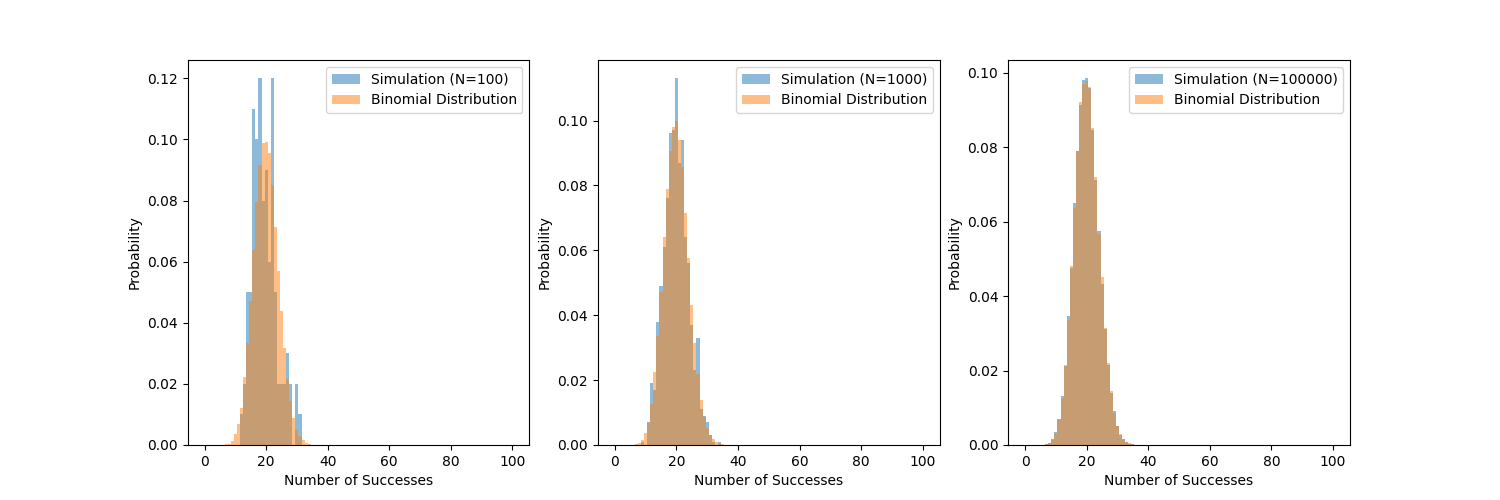
\includegraphics[width=\textwidth]{set1-p8.png}
	\caption{Histograms of the number of successes in 100 Bernoulli trials with $p=0.2$, for $N=100$, $N=1000$, and $N=100000$ pseudo-experiments. The blue bars are the results from the pseudo-experiments, and the orange is the normalized Binomial distribution histogram.}
	\label{fig:bernoulli}
\end{figure}

\subsection*{Problem 9}
\begin{quote}
	Prove that the correlation coefficient between any two variables satisfies $-1\le \rho(x,y)\le 1$.
\end{quote}

\divider

For this problem I followed the approach taken from \cite{statproofbook2023corr}. So full credit to them for the proof idea.

Consider the variance of the normalized sum or difference of $x$ and $y$:
\[
	\mathrm{Var}\!\left(\frac{x}{\sigma_x} \pm \frac{y}{\sigma_y}\right),
\]
where $\sigma_x$ and $\sigma_y$ are the standard deviations of $x$ and $y$, respectively.

Since variance is always non-negative, we have
\[
	0 \le \mathrm{Var}\!\left(\frac{x}{\sigma_x} \pm \frac{y}{\sigma_y}\right).
\]

Expanding the variance of a linear combination gives
\[
	\mathrm{Var}\!\left(\frac{x}{\sigma_x} \pm \frac{y}{\sigma_y}\right)
	= \mathrm{Var}\!\left(\frac{x}{\sigma_x}\right) + \mathrm{Var}\!\left(\frac{y}{\sigma_y}\right) \pm 2\,\mathrm{Cov}\!\left(\frac{x}{\sigma_x}, \frac{y}{\sigma_y}\right)
	= 1 + 1 \pm 2\,\rho(x,y),
\]
where we used $\mathrm{Var}(x/\sigma_x) = 1$ and $\mathrm{Cov}(x/\sigma_x, y/\sigma_y) = \rho(x,y)$, the correlation coefficient.

Thus,
\[
	0 \le 2 \pm 2 \,\rho(x,y),
\]
which simplifies to
\[
	-1 \le \rho(x,y) \le 1.
\]

\hfill $\square$







\subsection*{Problem 10}
\begin{quote}
	Suppose you measure the position of an object on a plane as $(x,y)$, with uncertainties on the measurements $\sigma_x$, $\sigma_y$ that are uncorrelated. If you express the position in polar coordinates $(r,\theta)$ with $x=r\cos\theta$, $y=r\sin\theta$, what is the covariance matrix $V(r,\theta)$? Under what conditions is the covariance (and hence the correlation coefficient) between $r,\theta$ zero? When is it positive, and when negative? Draw sketches of the measurement uncertainty ellipses in the various cases to demonstrate the answer.
\end{quote}

\divider

Recall that for $\vec{z} = f(\vec{x})$, the Jacobian matrix $J$ has elements:

\[ J_{ij} = \frac{\partial z_i}{\partial x_j} \]

Here we have $r = \sqrt{x^2 + y^2}$ and $\theta = \tan^{-1}(y/x)$. So we can then compute the Jacobian J of the transformation from Cartesian to polar coordinates

\[ J = \begin{bmatrix}
		\pdv{r}{x}      & \pdv{r}{y}      \\
		\pdv{\theta}{x} & \pdv{\theta}{y}
	\end{bmatrix} \]

Using $r = \sqrt{x^2 + y^2}$, and $\theta = \tan^{-1}(y/x)$, we can compute the partial derivatives (using WA):

\[ \pdv{r}{x} = x / \sqrt{x^2 + y^2} \]
\[ \pdv{r}{y} = y / \sqrt{x^2 + y^2} \]
\[ \pdv{\theta}{x} = -y / (x^2 + y^2) \]
\[ \pdv{\theta}{y} = x / (x^2 + y^2) \]


\[ J = \begin{bmatrix}
		\frac{x}{\sqrt{x^2 + y^2}} & \frac{y}{\sqrt{x^2 + y^2}} \\
		-\frac{y}{x^2 + y^2}       & \frac{x}{x^2 + y^2}
	\end{bmatrix} \]

Since $x = r\cos\theta$ and $y = r\sin\theta$, we can rewrite the Jacobian in terms of $r$ and $\theta$:

\[ J = \begin{bmatrix}
		\cos\theta    & \sin\theta   \\
		-\sin\theta/r & \cos\theta/r
	\end{bmatrix} \]

From that we can use the general transformation of covariance matrices formula:

\[ V_z \approx J V_x J^T \]

\[ V_{r,\theta} \approx J V(x,y) J^T \]

Since measurements of $x$ and $y$ are uncorrelated, the covariance matrix $V(x,y)$ is just diagonal:

\[ V(x,y) = \begin{bmatrix}
		\sigma_x^2 & 0          \\
		0          & \sigma_y^2
	\end{bmatrix} \]

Then the covariance matrix in polar coordinates is:

\[ V(r,\theta) = J V(x,y) J^T \]

\[ V(r,\theta) = \begin{bmatrix}
		\cos\theta    & \sin\theta   \\
		-\sin\theta/r & \cos\theta/r
	\end{bmatrix}\begin{bmatrix}
		\sigma_x^2 & 0          \\
		0          & \sigma_y^2
	\end{bmatrix} \begin{bmatrix}
		\cos\theta    & \sin\theta   \\
		-\sin\theta/r & \cos\theta/r
	\end{bmatrix}^T\]



\[
	\boxed{V(r,\theta) =
		\begin{bmatrix}
			\sigma_x^2\cos^2\theta + \sigma_y^2\sin^2\theta       & \frac{(\sigma_y^2-\sigma_x^2)\cos\theta\sin\theta}{r}       \\
			\frac{(\sigma_y^2-\sigma_x^2)\cos\theta\sin\theta}{r} & \frac{\sigma_y^2\cos^2\theta + \sigma_x^2\sin^2\theta}{r^2}
		\end{bmatrix}}
\]

\begin{itemize}
	\item We can determine when the covariance between $r$ and $\theta$ is zero by setting the off-diagonal terms to zero.

	      \[ \text{Cov}(r,\theta) = \dfrac{(\sigma_y^2-\sigma_x^2)\cos\theta\sin\theta}{r} = 0 \]
	      \begin{itemize}
		      \item First we see that if $\sigma_x^2 = \sigma_y^2 = \sigma^2$, then the off-diagonal terms are zero, and hence the covariance is zero (and Var$(r) = \sigma^2$ and Var$(\theta) = \sigma^2/r^2$).
		      \item The covariance is also zero when $\cos\theta\sin\theta = 0$, which occurs when $\theta = n\pi/2$ for integer $n$. This corresponds to the cases where the point lies on the x or y axis.
	      \end{itemize}
	\item The covariance is positive or negative depending on the sign of the off-diagonal terms:

	      If $\sin\theta\cos\theta < 0$ (second and third quadrants):
	      \begin{itemize}
		      \item When $\sigma_y^2 > \sigma_x^2$, the covariance is negative.
		      \item When $\sigma_y^2 < \sigma_x^2$, the covariance is positive.
	      \end{itemize}
	      If $\sin\theta\cos\theta > 0$ (first and fourth quadrants):
	      \begin{itemize}
		      \item When $\sigma_y^2 > \sigma_x^2$, the covariance is positive.
		      \item When $\sigma_y^2 < \sigma_x^2$, the covariance is negative.
	      \end{itemize}
\end{itemize}

Sketches of the measurement uncertainty ellipses in the various cases to demonstrate the answer.

\begin{figure}
	\centering
	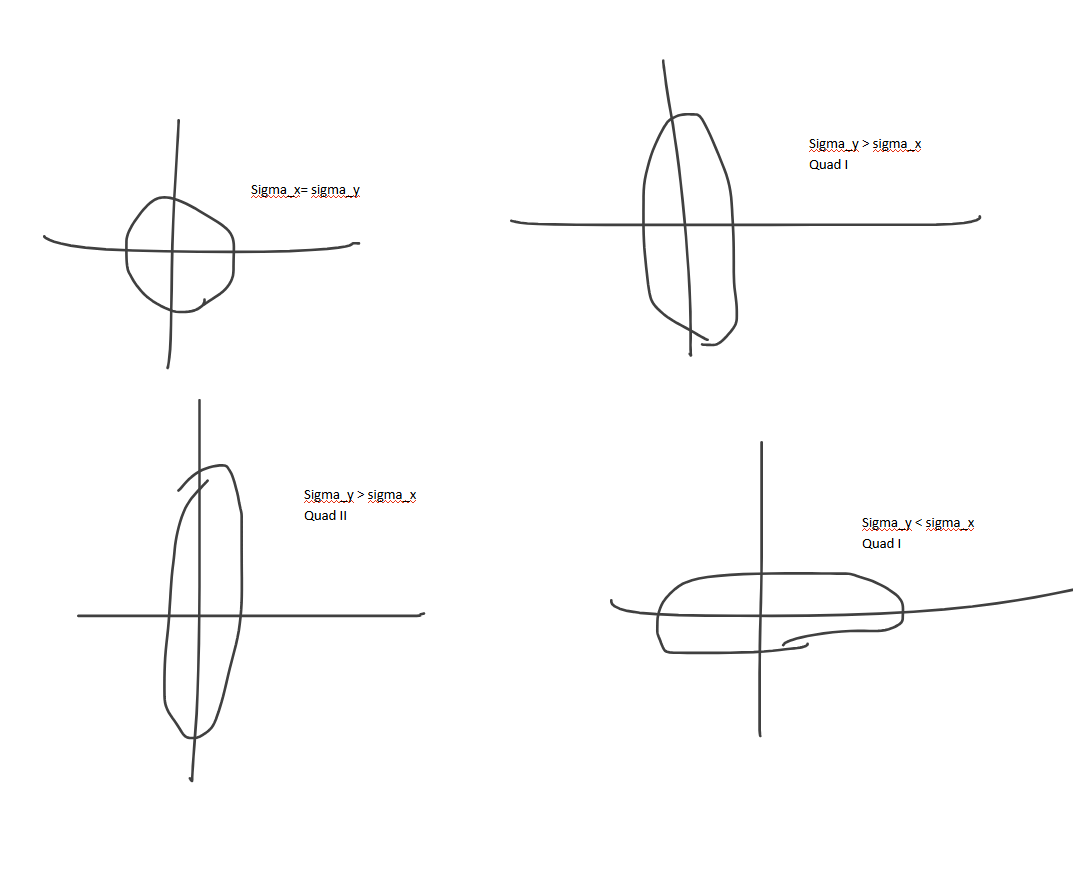
\includegraphics[width=\textwidth]{set1-p10.png}
	\caption{Measurement uncertainty ellipses for various cases of $\sigma_x$, $\sigma_y$, and $\theta$ (quadrant indicated)}
	\label{fig:ellipses}
\end{figure}



\subsection*{Problem 11}
\begin{quote}
	Given uncorrelated original probability densities for $x,y$ (i.e., $V_{ij}=\operatorname{diag}(\sigma_x^2,\sigma_y^2)$), find $\sigma_z=\sqrt{V_z}$ for the following functional transformations:
	\begin{enumerate}[label=(\alph*)]
		\item $z=x^2$
		\item $z=\sin(a x)$, where $a$ is a constant
		\item $z=e^{-x/\tau}$, where $\tau$ is a constant
		\item $z=\log x$
		\item $z=x+y$
		\item $z=x-y$
		\item $z=x\,y$
		\item $z=x/y$
	\end{enumerate}
\end{quote}

\divider

Recall that for $\vec{z} = f(\vec{x})$, the Jacobian matrix $J$ has elements:

\[ J_{ij} = \frac{\partial z_i}{\partial x_j} \]

Then we can use the general transformation of covariance matrices formula again:

\[ V_z \approx J V_x J^T \]


In this question we have a scalar case where we just have one output variable $z$, and here there is examples with both 1 or 2 input variables ($x$ and sometimes $y$). So the Jacobian matrix is either a 1x1 matrix or a 2x1 matrix.

\begin{itemize}
	\item For the case of 1 varaible input ($x$ only), the Jacobian is:

	      \[ J = \begin{bmatrix}
			      \pdv{z}{x}
		      \end{bmatrix} = \pdv{z}{x} \]

	      And then the covariance matrix of $z$ is:

	      \[ V_z = J V_x J^T = \pdv{z}{x} \sigma_x^2 \pdv{z}{x} = \left(\pdv{z}{x}\right)^2 \sigma_x^2 \]

	\item For the case of 2 variable input ($x$ and $y$), the Jacobian is:

	      \[ J = \begin{bmatrix}
			      \pdv{z}{x} & \pdv{z}{y}
		      \end{bmatrix} \]


	      And then the covariance matrix of $z$ is:
	      \[ V_z = J V_x J^T = \begin{bmatrix}
			      \pdv{z}{x} & \pdv{z}{y}
		      \end{bmatrix} \begin{bmatrix}
			      \sigma_x^2 & 0          \\
			      0          & \sigma_y^2
		      \end{bmatrix} \begin{bmatrix}
			      \pdv{z}{x} & \pdv{z}{y}
		      \end{bmatrix}^T =
		      \left(\pdv{z}{x}\right)^2 \sigma_x^2 + \left(\pdv{z}{y}\right)^2 \sigma_y^2
	      \]
\end{itemize}


So for solving for $\sigma_z$, we have the two cases:

\begin{enumerate}
	\item 1 variable input ($x$ only):
	      \[ \sigma_z = \sqrt{V_z} = \left|\pdv{z}{x}\right| \sigma_x \]

	\item 2 variable input ($x$ and $y$):
	      \[ \sigma_z = \sqrt{V_z} = \sqrt{\left(\pdv{z}{x}\right)^2 \sigma_x^2 + \left(\pdv{z}{y}\right)^2 \sigma_y^2} \]
\end{enumerate}


\begin{enumerate}[label=(\alph*)]
	\item $z=x^2$:
	      \[ \boxed{\sigma_z = 2|x| \sigma_x} \]

	\item $z=\sin(a x)$, where $a$ is a constant
	      \[ \boxed{\sigma_z = |a \cos(a x)| \sigma_x} \]

	\item $z=e^{-x/\tau}$, where $\tau$ is a constant
	      \[ \boxed{\sigma_z = \frac{1}{\tau} e^{-x/\tau} \sigma_x} \]

	\item $z=\log x$
	      \[ \boxed{\sigma_z = \frac{1}{x} \sigma_x} \]

	\item $z=x+y$
	      \[ \boxed{\sigma_z = \sqrt{\sigma_x^2 + \sigma_y^2}} \]

	\item $z=x-y$
	      \[ \boxed{\sigma_z = \sqrt{\sigma_x^2 + \sigma_y^2}} \]

	\item $z=x\,y$
	      \[ \boxed{\sigma_z = \sqrt{y^2 \sigma_x^2 + x^2 \sigma_y^2}} \]

	\item $z=\frac{x}{y}$
	      \[ \boxed{\sigma_z = \sqrt{\frac{\sigma_x^2}{y^2} + \frac{x^2 \sigma_y^2}{y^4}}} \]

\end{enumerate}





\subsection*{Problem 12}
\begin{quote}
	Suppose you measure the voltage $V$ across a resistor of resistance $R$, and you estimate the square roots of the variances of the underlying probability distributions of the measurements to be $\sigma_V$ and $\sigma_R$, respectively. We then estimate the power $P=V^2/R$ and current $I=V/R$.
	\begin{enumerate}[label=(\alph*)]
		\item Calculate the covariance matrix $V(P,I)$, starting from the covariance matrix $V(V,R)$ (sorry for the double use of the symbol $V$, but it should be clear from context which one is meant).
		\item You can also express $P=VI$. So you could do the calculation in two steps: first calculate $I$, then calculate $P$ from $V$ and $I$, rather than from $V$ and $R$. Do this (i.e., first transform from $(V,R)$ to $(V,I)$, then transform those variables to $(P,I)$) and compare the final covariance matrix you get this way with the direct transformation.
	\end{enumerate}
\end{quote}

\divider

\begin{enumerate}[label=(\alph*)]
	\item To start we will get the covariance matrix $V(V,R)$:

	      \[ V(V,R) = \begin{bmatrix}
			      \sigma_V^2      & \text{Cov}(V,R) \\
			      \text{Cov}(R,V) & \sigma_R^2
		      \end{bmatrix} \]

	      Now let's build the transformation Jacobian matrix:

	      \[ J_{ij} = \frac{\partial z_i}{\partial x_j} \]

	      Where $\vec{z} = (P,I)$ and $\vec{x} = (V,R)$.

	      \[ J = \begin{bmatrix}
			      \pdv{P}{V} & \pdv{P}{R} \\
			      \pdv{I}{V} & \pdv{I}{R}
		      \end{bmatrix} \]

	      \[ J = \begin{bmatrix}
			      \frac{2V}{R} & -\frac{V^2}{R^2} \\
			      \frac{1}{R}  & -\frac{V}{R^2}
		      \end{bmatrix} \]
	      Now we can use the general transformation of covariance matrices formula:

	      \[ V(P,I) = J V(V,R) J^T \]

	      \[ V(P,I) = \begin{bmatrix}
			      \frac{2V}{R} & -\frac{V^2}{R^2} \\
			      \frac{1}{R}  & -\frac{V}{R^2}
		      \end{bmatrix}  \begin{bmatrix}
			      \sigma_V^2      & \text{Cov}(V,R) \\
			      \text{Cov}(R,V) & \sigma_R^2
		      \end{bmatrix} \begin{bmatrix}
			      \frac{2V}{R} & -\frac{V^2}{R^2} \\
			      \frac{1}{R}  & -\frac{V}{R^2}
		      \end{bmatrix}^T \]


	      Note that the covariance matrix is symmetric such that $\text{Cov}(V,R) = \text{Cov}(R,V) $.


	      \[ V(P,I) = \begin{bmatrix} \frac{2V}{R}\sigma_V^2 - \frac{V^2}{R^2}\text{Cov}(R,V) & \frac{2V}{R}\text{Cov}(V,R) - \frac{V^2}{R^2}\sigma_R^2 \\ \frac{1}{R}\sigma_V^2 - \frac{V}{R^2}\text{Cov}(R,V) & \frac{1}{R}\text{Cov}(V,R) - \frac{V}{R^2}\sigma_R^2 \end{bmatrix} \begin{bmatrix} \frac{2V}{R} & \frac{1}{R} \\ -\frac{V^2}{R^2} & -\frac{V}{R^2} \end{bmatrix} \]

	      \[
		      \boxed{ V(P,I) =
			      \begin{bmatrix}
				      \frac{4V^2}{R^2}\sigma_V^2 - \frac{4V^3}{R^3}\text{Cov}(R,V) + \frac{V^4}{R^4}\sigma_R^2 & \frac{2V}{R^2}\sigma_V^2 - \frac{3V^2}{R^3}\text{Cov}(R,V) + \frac{V^3}{R^4}\sigma_R^2 \\
				      \frac{2V}{R^2}\sigma_V^2 - \frac{3V^2}{R^3}\text{Cov}(R,V)  + \frac{V^3}{R^4}\sigma_R^2  & \frac{1}{R^2}\sigma_V^2 - \frac{2V}{R^3}\text{Cov}(R,V) + \frac{V^2}{R^4}\sigma_R^2
			      \end{bmatrix} }
	      \]

	\item To start we will need to get the covariance matrix of (V,I) for $I=V/R$ from (V,R):
	      \[ V(V,I) = J V(V,R) J^T \]

	      To start we just need to build the transformation Jacobian matrix:

	      \[ J_{ij} = \frac{\partial z_i}{\partial x_j} \]

	      Where $\vec{z} = (V,I)$ and $\vec{x} = (V,R)$. Where $I = V/R$ and $V = V$ (need to find equations for V and I in terms of only V and R).

	      \[ J = \begin{bmatrix}
			      \pdv{V}{V} & \pdv{V}{R} \\
			      \pdv{I}{V} & \pdv{I}{R}
		      \end{bmatrix} \]

	      \[ J = \begin{bmatrix}
			      1           & 0              \\
			      \frac{1}{R} & -\frac{V}{R^2}
		      \end{bmatrix} \]




	      As we saw before the covariance matrix $V(V,R)$ is:

	      \[ V(V,R) = \begin{bmatrix}
			      \sigma_V^2      & \text{Cov}(V,R) \\
			      \text{Cov}(R,V) & \sigma_R^2
		      \end{bmatrix} \]

	      So we can compute $V(V,I)$:

	      \[ V(V,I) = \begin{bmatrix}
			      1           & 0              \\
			      \frac{1}{R} & -\frac{V}{R^2}
		      \end{bmatrix}\begin{bmatrix}
			      \sigma_V^2      & \text{Cov}(V,R) \\
			      \text{Cov}(R,V) & \sigma_R^2
		      \end{bmatrix} \begin{bmatrix}
			      1           & 0              \\
			      \frac{1}{R} & -\frac{V}{R^2}
		      \end{bmatrix}^T \]


	      \[ V(V,I) = \begin{bmatrix}
			      \sigma_V^2                                           & \text{Cov}(V,R)                                      \\
			      \frac{1}{R}\sigma_V^2 - \frac{V}{R^2}\text{Cov}(R,V) & \frac{1}{R}\text{Cov}(V,R) - \frac{V}{R^2}\sigma_R^2
		      \end{bmatrix} \begin{bmatrix}
			      1 & \frac{1}{R}    \\
			      0 & -\frac{V}{R^2}
		      \end{bmatrix} \]


	      \[ V(V,I) = \begin{bmatrix} \sigma_V^2                                           & \frac{1}{R}\sigma_V^2 - \frac{V}{R^2}\text{Cov}(R,V)                                                               \\
                \frac{1}{R}\sigma_V^2 - \frac{V}{R^2}\text{Cov}(R,V) & \frac{1}{R^2} \sigma_V^2 - \frac{V}{R^3}\text{Cov}(R,V) - \frac{V}{R^3}\text{Cov}(V,R) + \frac{V^2}{R^4}\sigma_R^2
		      \end{bmatrix} \]
	      Now we have the covariance matrix $V(V,I)$, we can now transform to $V(P,I)$ where $P = V I$ and $I = I$ (need to find equations for P and I in terms of only V and I).

	      \[ V(P,I) = J V(V,I) J^T \]

	      \[ J = \begin{bmatrix}
			      \pdv{P}{V} & \pdv{P}{I} \\
			      \pdv{I}{V} & \pdv{I}{I}
		      \end{bmatrix} \]

	      \[ J = \begin{bmatrix}
			      I & V \\
			      0 & 1
		      \end{bmatrix} \]

	      So we can compute $V(P,I)$:

	      \[ V(P,I) = \begin{bmatrix}
			      I & V \\
			      0 & 1
		      \end{bmatrix}
		      \begin{bmatrix} \sigma_V^2                                           & \frac{1}{R}\sigma_V^2 - \frac{V}{R^2}\text{Cov}(R,V)                                                               \\
                \frac{1}{R}\sigma_V^2 - \frac{V}{R^2}\text{Cov}(R,V) & \frac{1}{R^2} \sigma_V^2 - \frac{V}{R^3}\text{Cov}(R,V) - \frac{V}{R^3}\text{Cov}(V,R) + \frac{V^2}{R^4}\sigma_R^2
		      \end{bmatrix} \begin{bmatrix}
			      I & V \\
			      0 & 1
		      \end{bmatrix}^T \]

	      \[
		      V(P,I)=
		      \begin{bmatrix}
			      A & B \\[4pt]
			      C & D
		      \end{bmatrix}
		      \begin{bmatrix}
			      I & 0 \\[2pt]
			      V & 1
		      \end{bmatrix}
	      \]
	      \begin{align*}
		      A & = I\sigma_V^2 + \frac{V}{R}\sigma_V^2 - \frac{V^2}{R^2}\operatorname{Cov}(R,V),                                      \\[6pt]
		      B & = \frac{I}{R}\sigma_V^2 - \frac{IV}{R^2}\operatorname{Cov}(R,V)
		      + \frac{V}{R^2}\sigma_V^2 - \frac{V^2}{R^3}\operatorname{Cov}(R,V)
		      - \frac{V^2}{R^3}\operatorname{Cov}(V,R) + \frac{V^3}{R^4}\sigma_R^2,                                                    \\[6pt]
		      C & = \frac{1}{R}\sigma_V^2 - \frac{V}{R^2}\operatorname{Cov}(R,V),                                                      \\[6pt]
		      D & = \frac{1}{R^2} \sigma_V^2 - \frac{V}{R^3}\text{Cov}(R,V) - \frac{V}{R^3}\text{Cov}(V,R) + \frac{V^2}{R^4}\sigma_R^2
	      \end{align*}


	      \[ V(P,I) = \begin{bmatrix} AI + BV & B \\ C I + D V & D \end{bmatrix} \]


	      \begin{align*}
		      AI + BV & = I^2\sigma_V^2 + \frac{I V}{R}\sigma_V^2 - \frac{I V^2}{R^2}\operatorname{Cov}(R,V) \\
		              & \quad + \frac{IV}{R}\sigma_V^2 - \frac{IV^2}{R^2}\operatorname{Cov}(R,V)
		      + \frac{V^2}{R^2}\sigma_V^2 - \frac{V^3}{R^3}\operatorname{Cov}(R,V)
		      - \frac{V^3}{R^3}\operatorname{Cov}(V,R) + \frac{V^4}{R^4}\sigma_R^2,
	      \end{align*}

	      Sub in $I = V/R$:

	      \[ AI +BV = \frac{4V^2}{R^2} \sigma_V^2 - \frac{4V^3}{R^3}\text{Cov}(R,V) + \frac{V^4}{R^4}\sigma_R^2 \]

	      Same for other terms:
	      \[ C I + DV = \frac{2V}{R^2}\sigma_V^2 - \frac{3V^2}{R^3}\text{Cov}(R,V) + \frac{V^3}{R^4}\sigma_R^2 \]
	      \[ B = \frac{2V}{R^2}\sigma_V^2 - \frac{3V^2}{R^3}\text{Cov}(R,V) + \frac{V^3}{R^4}\sigma_R^2 \]
	      \[ D = \frac{1}{R^2}\sigma_V^2 - \frac{2V}{R^3}\text{Cov}(R,V) + \frac{V^2}{R^4}\sigma_R^2 \]

	      \[ \boxed{V(P,I) = \begin{bmatrix} \frac{4V^2}{R^2}\sigma_V^2 - \frac{4V^3}{R^3}\text{Cov}(R,V) + \frac{V^4}{R^4}\sigma_R^2 & \frac{2V}{R^2}\sigma_V^2 - \frac{3V^2}{R^3}\text{Cov}(R,V) + \frac{V^3}{R^4}\sigma_R^2 \\ \frac{2V}{R^2}\sigma_V^2 - \frac{3V^2}{R^3}\text{Cov}(R,V)  + \frac{V^3}{R^4}\sigma_R^2  & \frac{1}{R^2}\sigma_V^2 - \frac{2V}{R^3}\text{Cov}(R,V) + \frac{V^2}{R^4}\sigma_R^2 \end{bmatrix} }\]

	      Which is the same result as part (a).
\end{enumerate}

\subsection*{Problem 13 The Geometric Distribution}
\begin{quote}
	Consider a Bernoulli process with probability of success in each trial being $p$.
	\begin{enumerate}[label=(\alph*)]
		\item Show that the probability that the first success occurs on the $n$th trial is given by the geometric distribution
		      \[
			      P_1(n;p) = p\,(1-p)^{n-1}.
		      \]
		      Verify that this gives a properly normalized set of probabilities, i.e.,
		      \[
			      \sum_{n=1}^{\infty} P_1(n;p) = 1.
		      \]
		\item Show that the mean and variance of this distribution are
		      \[
			      E(r)=\frac{1}{p}, \qquad V(r)=\frac{1-p}{p^2}.
		      \]
		\item Make a plot of this distribution for $p=0.4$.
	\end{enumerate}
\end{quote}

\divider

\begin{enumerate}[label=(\alph*)]
	\item Let's take the sum:

	      \[ \sum _{n=1}^{\infty} P_1(n;p) = \sum_{n=1}^{\infty} p(1-p)^{n-1} = p \sum_{n=0}^{\infty} (1-p)^n \]

	      Since $|1-p| < 1$ for $0 < p < 1$, we can use the formula for the sum of an infinite geometric series:

	      \[ \sum_{n=0}^{\infty} (1-p)^n = \frac{1}{1-(1-p)} = \frac{1}{p} \]

	      So we have:

	      \[ \sum _{n=1}^{\infty} P_1(n;p) = p \cdot \frac{1}{p} = 1 \]


	\item To show the mean  we can use the formula for the expectation of an infinite geometric series:

	      \[ E(r) = \sum_{n=1}^{\infty} n P_1(n;p) = \sum_{n=1}^{\infty} n p (1-p)^{n-1} = p \sum_{n=1}^{\infty} n (1-p)^{n-1} \]

	      We can let $(1-p) = q$ for simplicity, and then we have:

	      \[ E(r) = p \sum_{n=1}^{\infty} n q^{n-1} \]

	      We can use the formula for the sum of an infinite geometric series that we covered in lecture 7:

	      \[ \sum_{n=1}^{\infty} n q^{n-1} = \frac{1}{(1-q)^2} \]


	      So we have:

	      \[ E(r) = p \frac{1}{(1-q)^2} = p \frac{1}{(1-1+p)^2} \]

	      \[ \boxed{E(r) = \frac{1}{p}} \]

	      To show variance we can use the definition of variance:

	      \[ V(r) = E(r^2) - (E(r))^2 \]

	      We already have $E(r)$, so we just need to compute $E(r^2)$:

	      \[ E(r^2) = \sum_{n=1}^{\infty} n^2 P_1(n;p) = \sum_{n=1}^{\infty} n^2 p (1-p)^{n-1} = p \sum_{n=1}^{\infty} n^2 (1-p)^{n-1} \]

	      Again let $(1-p) = q$ for simplicity, and then we have:

	      \[ E(r^2) = p \sum_{n=1}^{\infty} n^2 q^{n-1} \]

	      We can use the formula for the sum of an infinite geometric series that we covered in lecture 7:

	      \[ \sum_{n=1}^{\infty} n^2 q^{n-1} = \frac{1+q}{(1-q)^3} \]

	      So we have:

	      \[ E(r^2) = p \frac{1+q}{(1-q)^3} = p \frac{1 + 1 - p}{(p)^3} = p \frac{2 - p}{p^3} = \frac{2 - p}{p^2} \]

	      Now we can compute the variance:

	      \[ V(r) = E(r^2) - (E(r))^2 = \frac{2 - p}{p^2} - \left(\frac{1}{p}\right)^2 = \frac{2 - p - 1}{p^2} = \frac{1 - p}{p^2} \]

	      \[ \boxed{V(r) = \frac{1 - p}{p^2}} \]


	\item See figure \ref{fig:geometric}. Source code to generate the plot (credit to github copilot for code suggestions):


	      \begin{verbatim}
		import numpy as np
		import matplotlib.pyplot as plt
		import scienceplots

		plt.style.use(['science', 'notebook'])

		p = 0.4  # probability of success
		n = np.arange(1, 19)  # number of trials
		P1 = p * (1 - p) ** (n - 1)  # geometric distribution
		P1 /= np.sum(P1)  # normalize probabilities

		plt.bar(n, P1, label='Geometric Distribution (p=0.4)')
		plt.xlabel('Number of Trials (n)')
		plt.ylabel('Probability')
		plt.legend()



		path = 'C:/Users/tobia/Documents/ubc-grad/PHYS509-UBC-TheoryofMeasurements-notes/homework-problems/problem-set-1/'
		plt.savefig(f'{path}set1-p13c.png')
		plt.show()
	\end{verbatim}

	      \begin{figure}[h]
		      \centering
		      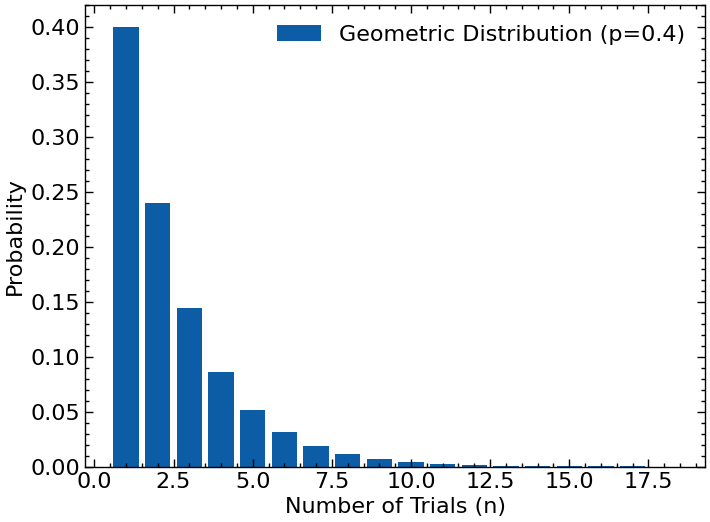
\includegraphics[width=0.7\textwidth]{set1-p13c.png}
		      \caption{Plot of the geometric distribution for $p=0.4$.}
		      \label{fig:geometric}
	      \end{figure}



\end{enumerate}

% r−1

\subsection*{Problem 14 The Negative Binomial Distribution}
\begin{quote}
	Suppose, instead of the usual binomial situation in which we fix the number of trials $n$ and ask how many successes $r$ we get, we reverse the problem: we keep performing trials until we get $r$ successes and ask how many trials $n$ we had to make.
	\begin{enumerate}[label=(\alph*)]
		\item Generalize the argument for the geometric distribution to show that the probability that the $r$th success is on the $n$th trial is given by the negative binomial distribution
		      \[
			      P_r(n;p) = {n-1 \choose r-1}\, p^r (1-p)^{n-r}, \qquad n=r, r+1,\ldots
		      \]

		\item Show that the mean and variance of this distribution are
		      \[
			      E(n)=\frac{r}{p}, \qquad V(n)=\frac{r(1-p)}{p^2}.
		      \]
		\item Make a plot of this distribution for $p=0.4,\ r=10$ and for $p=0.6,\ r=5$.
	\end{enumerate}
\end{quote}

\divider

\begin{enumerate}[label=(\alph*)]
	\item Each trial has p probability of success. Looking at r successes in n trials. The last trial must be a success, and the previous n-1 trials must contain r-1 successes. The number of ways to arrange r-1 successes in n-1 trials is given by the binomial coefficient:

	      \[ {n-1 \choose r-1} = \frac{(n-1)!}{(r-1)!(n-r)!} \]

	      The probability of getting r-1 successes and n-r failures in the first n-1 trials is:

	      \[ p^{r-1} (1-p)^{n-r} \]

	      The probability of getting a success on the nth trial is p. So the total probability of getting r successes in n trials is:

	      \[ P_r(n;p) = {n-1 \choose r-1} p^{r-1} (1-p)^{n-r} p \]
	      \[ \boxed{P_r(n;p)= {n-1 \choose r-1} p^r (1-p)^{n-r}} \]


	\item We can note that n is a sum of r independent geometric random variables. Each geometric random variable has mean \( \frac{1}{p} \) and variance \( \frac{1-p}{p^2} \). Therefore, we have:
	      \[\boxed{E(n) = r \cdot \frac{1}{p} }\]
	      \[\boxed{V(n) = r \cdot \frac{1-p}{p^2} }\]

	      Where r=1 is the geometric distribution.
	\item See figure \ref{fig:negative-binomial}. Source code to generate the plot (credit to github copilot for code suggestions):

	      \begin{verbatim}
	
	import numpy as np
	import matplotlib.pyplot as plt
	import scienceplots
	from scipy.special import comb

	plt.style.use(['science', 'notebook'])

	cases = [(0.4, 10), (0.6, 5)]  # (p, r) pairs

	plt.figure(figsize=(10, 5))

	for i, (p, r) in enumerate(cases, start=1):
		n = np.arange(r, 60)  # number of trials
		P_r = comb(n-1, r-1) * (p**r) * ((1-p)**(n-r))  # negative binomial distribution
		P_r /= np.sum(P_r)  # normalize for plotting

		plt.subplot(1, 2, i)
		plt.bar(n, P_r, alpha=0.7, label=f'p={p}, r={r}')
		plt.xlabel('Number of Trials (n)')
		plt.ylabel('Probability')
		plt.legend()

	path = 'C:/Users/tobia/Documents/ubc-grad/PHYS509-UBC-TheoryofMeasurements-notes/homework-problems/problem-set-1/'
	plt.tight_layout()
	plt.savefig(f'{path}set1-p14c.png')
	plt.show()

	\end{verbatim}

	      \begin{figure}[h]
		      \centering
		      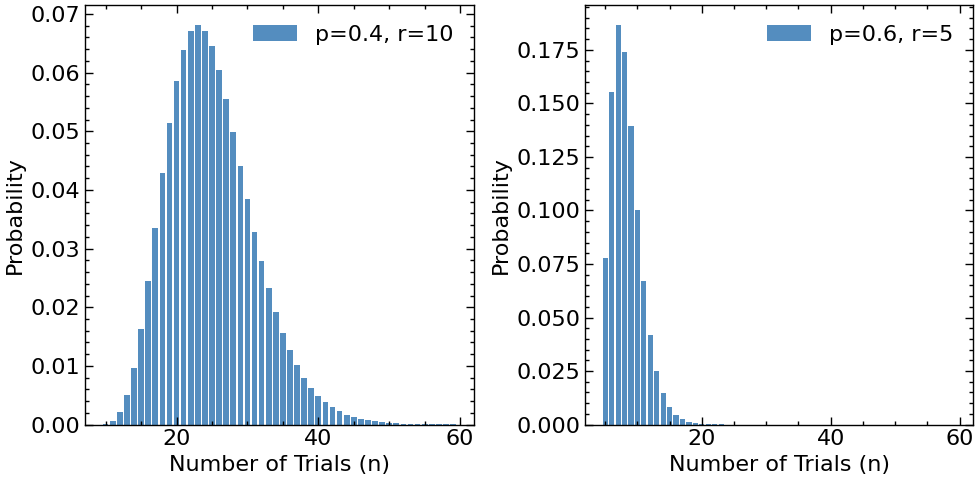
\includegraphics[width=0.7\textwidth]{set1-p14c.png}
		      \caption{Plot of the negative binomial distribution for $p=0.4, r=10$ and $p=0.6, r=5$.}
		      \label{fig:negative-binomial}
	      \end{figure}
\end{enumerate}


\printbibliography


\end{document}

